\documentclass[tikz]{standalone}
\usepackage{pgfplots}
\pgfplotsset{compat=1.18} % Use a recent compatibility version
\usepgfplotslibrary{colormaps}

\begin{document}
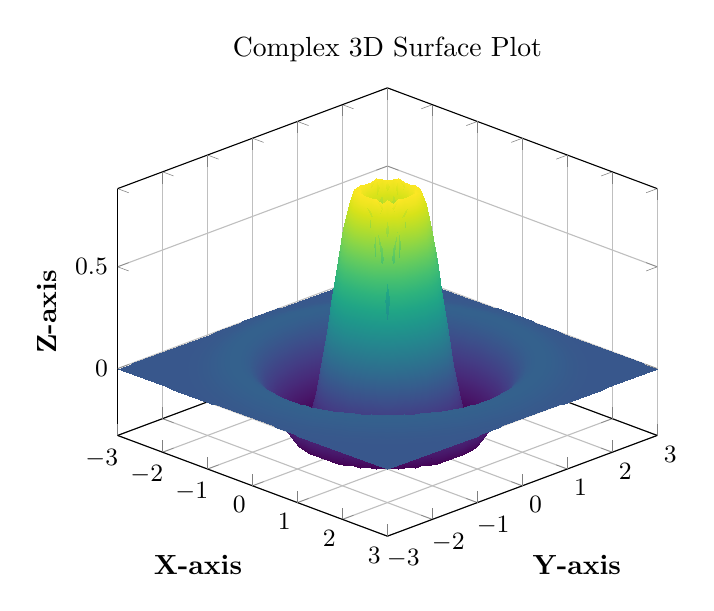
\begin{tikzpicture}
    \begin{axis}[
        title={Complex 3D Surface Plot},
        xlabel={X-axis},
        ylabel={Y-axis},
        zlabel={Z-axis},
        view={45}{30}, % Adjust view angles for better perspective
        colormap/viridis, % Use a visually appealing colormap
        % Add grid lines for better readability
        grid=major,
        tick label style={font=\small},
        label style={font=\bfseries},
        enlargelimits=false, 
        % Customize tick marks
        xtick distance=1,
        ytick distance=1,
        ztick distance=0.5,
    ]
    \addplot3[
        surf, 
        samples=50, 
        domain=-3:3, 
        domain y=-3:3, 
        z buffer=sort, 
        faceted color=mapped color, 
        shader=interp, 
        line width=0.3pt, % Thin colored mesh lines
    ]
    {exp(-(x^2+y^2)/2) * sin(deg(sqrt(x^2+y^2)*3))}; 
    \end{axis}
\end{tikzpicture}
\end{document}

